
\section{Materials and Methods}

\subsection{Small Radio Telescope (SRT)}
All measurements were performed using the small radio telescope located on top of the ExWi building.
It has a parabolic dish with a diameter of \SI{4}{m} and a feedhorn antenna. This causes main and side lobes, where the shape of the main lobe can be approximated as Gaussian.

\subsubsection{Signal Processing}
\begin{figure}[H]
    \centering
    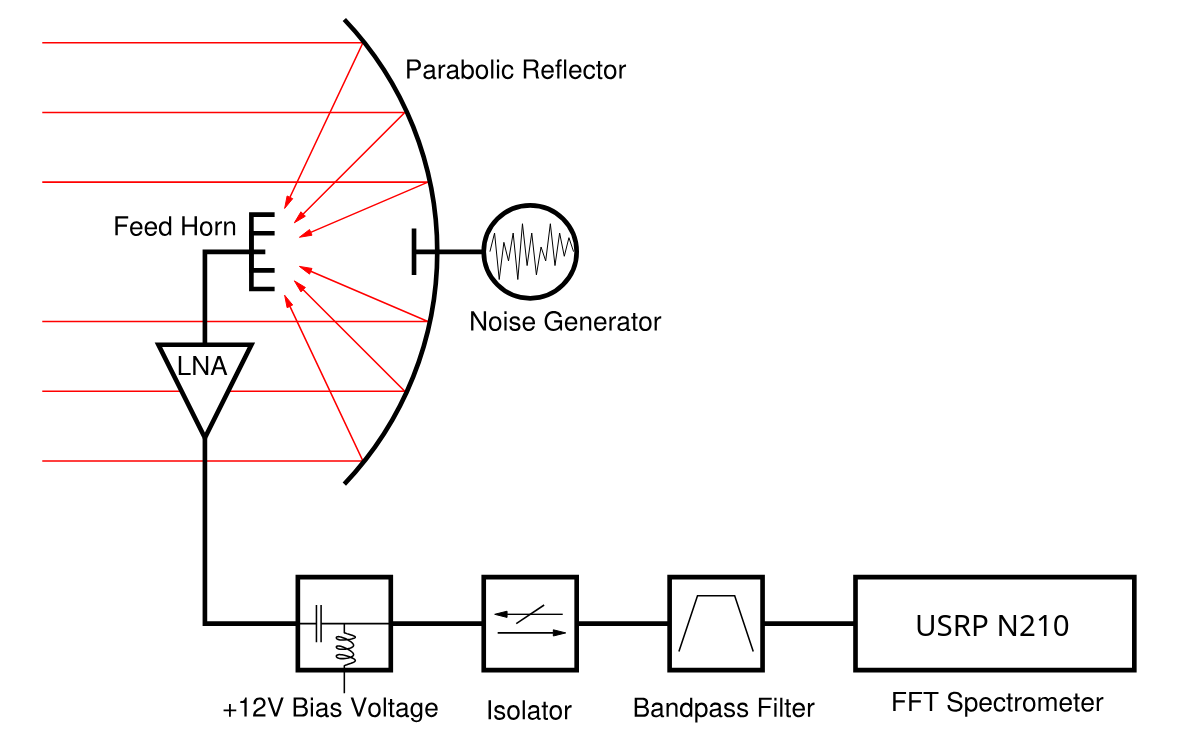
\includegraphics[width=0.6\textwidth]{assets/schematic.png}
    \caption{Schematic of the signal process. \cite[Fig. 3]{srt} hTODO: FIX THE SCHEMATIC}
    \label{fig:signal}
\end{figure}
The signal processing is shown schematically in Figure \ref{fig:signal}.
After the radiowaves are focused by the parabolic dish and received by the feedhorn antenna, they are first amplified by a low noise amplifier (LNA).
The amplified signal is then transmitted through a coaxial cable into the laboratory, where it passes through the receiver chain. This includes a bias-T that injects the supply voltage for the LNA,
a microwave isolator to prevent reflections, and a band-pass filter restricting the signal to the frequency range of \qtyrange{1.400}{1.427}{GHz}.
TODO: THE SQUARING CIRCUIT IS NOT IN THE SCHEMATIC, BUT SHOULD PROBABLY BE DESCRIBED HERE!
Finally, the filtered signal enters a digital spectrometer based on the \quote{Universal Software Defined Radio} (USRP) receiver,
where it is down-converted, digitized, and analyses using a Fast Fourier Transform (FFT). \cite[Sec. 4]{srt}

The outputs of the Fourier transform are spectral amplitude densities with units of [\si{\volt/\hertz}]. This value is proportional to the power density and its integration is proportional to the power.
This can lead to confusion if we denote axes in figures with units of Volts even though their physical interpretation should be as a value of Power.
For the rest of this report we will denote the unit of this amplitude in arbitrary units [\si{a.u.}] and the spectral amplitude density with units of [\si{a.u./\hertz}].
We will also use the symbol $P$ to denote such values to better convey the physical meaning.

\subsection{Lab View Tool}
sketch, description


\subsection{Measurement data and Code}
All data and code used in this report are available in a public repository\footnote{\url{https://github.com/SecretGmG/lab/tree/main/srt}}.

Error propagation and data fitting were performed using the publicly available module PhysicsTool\footnote{\url{https://github.com/SecretGmG/PhysicsTool}}.